% Created 2013-09-12 czw 02:13
\documentclass[presentation,aspectratio=43,12pt]{beamer}
\usepackage{fontspec}
\usepackage{fixltx2e}
\usepackage{graphicx}
\usepackage{longtable}
\usepackage{float}
\usepackage{wrapfig}
\usepackage[normalem]{ulem}
\usepackage{textcomp}
\usepackage{marvosym}
\usepackage{wasysym}
\usepackage{amssymb}
\usepackage{amstext}
\usepackage{hyperref}
\tolerance=1000
\usepackage{pgfpages}
\usepackage{tikz}
\institute[SRPOL]{Samsung R\&D Institute Poland}
\renewcommand\pgfsetupphysicalpagesizes{\pdfpagewidth\pgfphysicalwidth\pdfpageheight\pgfphysicalheight}
\AtBeginSection[]{{\setbeamertemplate{footline}{}\setbeamertemplate{background canvas}[section page]\begin{frame}<beamer>\sectionpage\end{frame}\setbeamertemplate{footline}[tizen]}}
\setbeameroption{show notes on second screen=bottom}
\hypersetup{colorlinks=true,linkcolor=,urlcolor=pantone326}
\usetheme{smartdevcon2}
\author{Łukasz Stelmach}
\date{12–14 September, 2013}
\title{Tizen Architecture}
\hypersetup{
  pdfkeywords={},
  pdfsubject={},
  pdfcreator={Emacs 24.2.1 (Org mode 8.1.1)}}
\begin{document}

\maketitle
\begin{frame}{Outline}
\tableofcontents
\end{frame}



\note{T-43

Good morning everyone, my name is Łukasz Stelmach, I work for
Samsung R\&D Institute Poland and I am going to talk about Tizen,
some of its internals and externals.

Those of you who have followed Tizen development know probably more
than I will tell today. I hope, however, that the rest would find my
presentation interesting and educating.

Questions? Ask!}
\section{Introduction to Tizen}
\label{sec-2}
\note{Tizen isn't the most popular operating system yet, so I suppose a
brief introduciton will be helpful.}
\begin{frame}[label=sec-2-2]{Tizen}
\begin{itemize}
\item Open source
\begin{itemize}
\item GNU/Linux
\item WebKit
\item EFL
\end{itemize}
\item Standards-based
\begin{itemize}
\item POSIX
\item HTML5
\end{itemize}
\item Smart-embedded
\begin{itemize}
\item Phones
\item Tablets
\item IVI
\item TV
\end{itemize}
\end{itemize}

\note{T-40

\begin{itemize}
\item It has GNU/Linux basic userland
\item POSIX + HTML5
\item Smart-embedded devices
\end{itemize}}
\end{frame}
\begin{frame}[label=sec-2-3]{Family tree \tiny (\url{https://github.com/kumadasu/tizen-history})}
\begin{center}
\begin{tikzpicture}[x=1pt,y=1pt]
\note<1-2>{As you all probably know $\hookleftarrow$ Samsung Electronics has been
  making mobiles for quite some time. Some of theme were smarter than
  other.}

\fill<2->[fill=pantone2985]( 123.5pt,  86pt) ellipse (12.5pt and 6.26pt); % Samsung

\note<3>{In 2007, Samsung together with other manufacturers
  established LiMo Foundation. Its mission was to create an open,
  Linux-based software platform for mobile devices.
  http://www.theregister.co.uk/2007/01/26/limo\_founded/}
\fill<3->[fill=pantone2985](  76pt,  46pt) ellipse (15pt and 6.26pt); % LiMo Foundation

\note<4>{The foundation released two version of the platform with
  significant contribution ported from Samsung's SLP.}
\fill<4-6>[fill=pantone2985](  83.7pt,  32.5pt) ellipse (12.5pt and 6.26pt); % LiMo
\fill<4-6>[fill=pantone2985](  89.3pt, -34.0pt) ellipse (12.5pt and 6.26pt); % LiMo4
\fill<4-6>[fill=pantone2985]( 112.3pt,   6pt) ellipse (12.5pt and 6.26pt); % SLP

\note<5-6>{In the meantime, Intel, was working on its own Moblin
  distribution. It was later merged with Nokia's Maemo to form
  $\hookleftarrow$ MeeGo.}
\draw<6>[draw=pantone2985,line width=2pt]%
    ( -49.0,   -20.0) .. controls (-49,28) and (-37.7,28) .. (-37.4, 86);
\fill<5->[fill=pantone2985]( -36.7pt,  86pt) ellipse (12.5pt and 6.26pt); % Intel
\fill<6>[fill=pantone2985]( -49.0pt, -20.5pt) ellipse (12.5pt and 6.26pt); % MeeGo 1.2

\note<7-9>{Shortly after releasing version 1.2, Intel decided to
  discontinue developemnt of MeeGo, and join LiMo Foundation which, at
  the same time, together with $\hookleftarrow$ Linux Foundation,
  announced a new project named Tizen. Few months later LiMo
  Foundation changed its name to $\hookleftarrow$ Tizen Association.}
\fill<8->[fill=pantone2985]( 101,  86) ellipse (12.5pt and 6.26pt); % Linux Foundation
\fill<9->[fill=pantone2985](  66.3pt, -34.0pt) ellipse (15pt and 6.26pt); % Tizen Association

\note<10-11>{In 2012, the first version of Tizen SDK was released
  $\hookleftarrow$ followed by versions 2.0 and 2.2 in 2013, which
  provide official Native API from Samsung's Bada. }
\fill<10->[fill=pantone2985]( 105.1pt, -47.0pt) ellipse (25pt and 6.26pt); % Tizen 1.0
\fill<10->[fill=pantone2985]( 5.0pt, -47.0pt) ellipse (20pt and 6.26pt); % Tizen IVI
\fill<11->[fill=pantone2985]( 123.5pt, -87.0pt) ellipse (25pt and 6.26pt); % Tizen 2.0
\pgftext{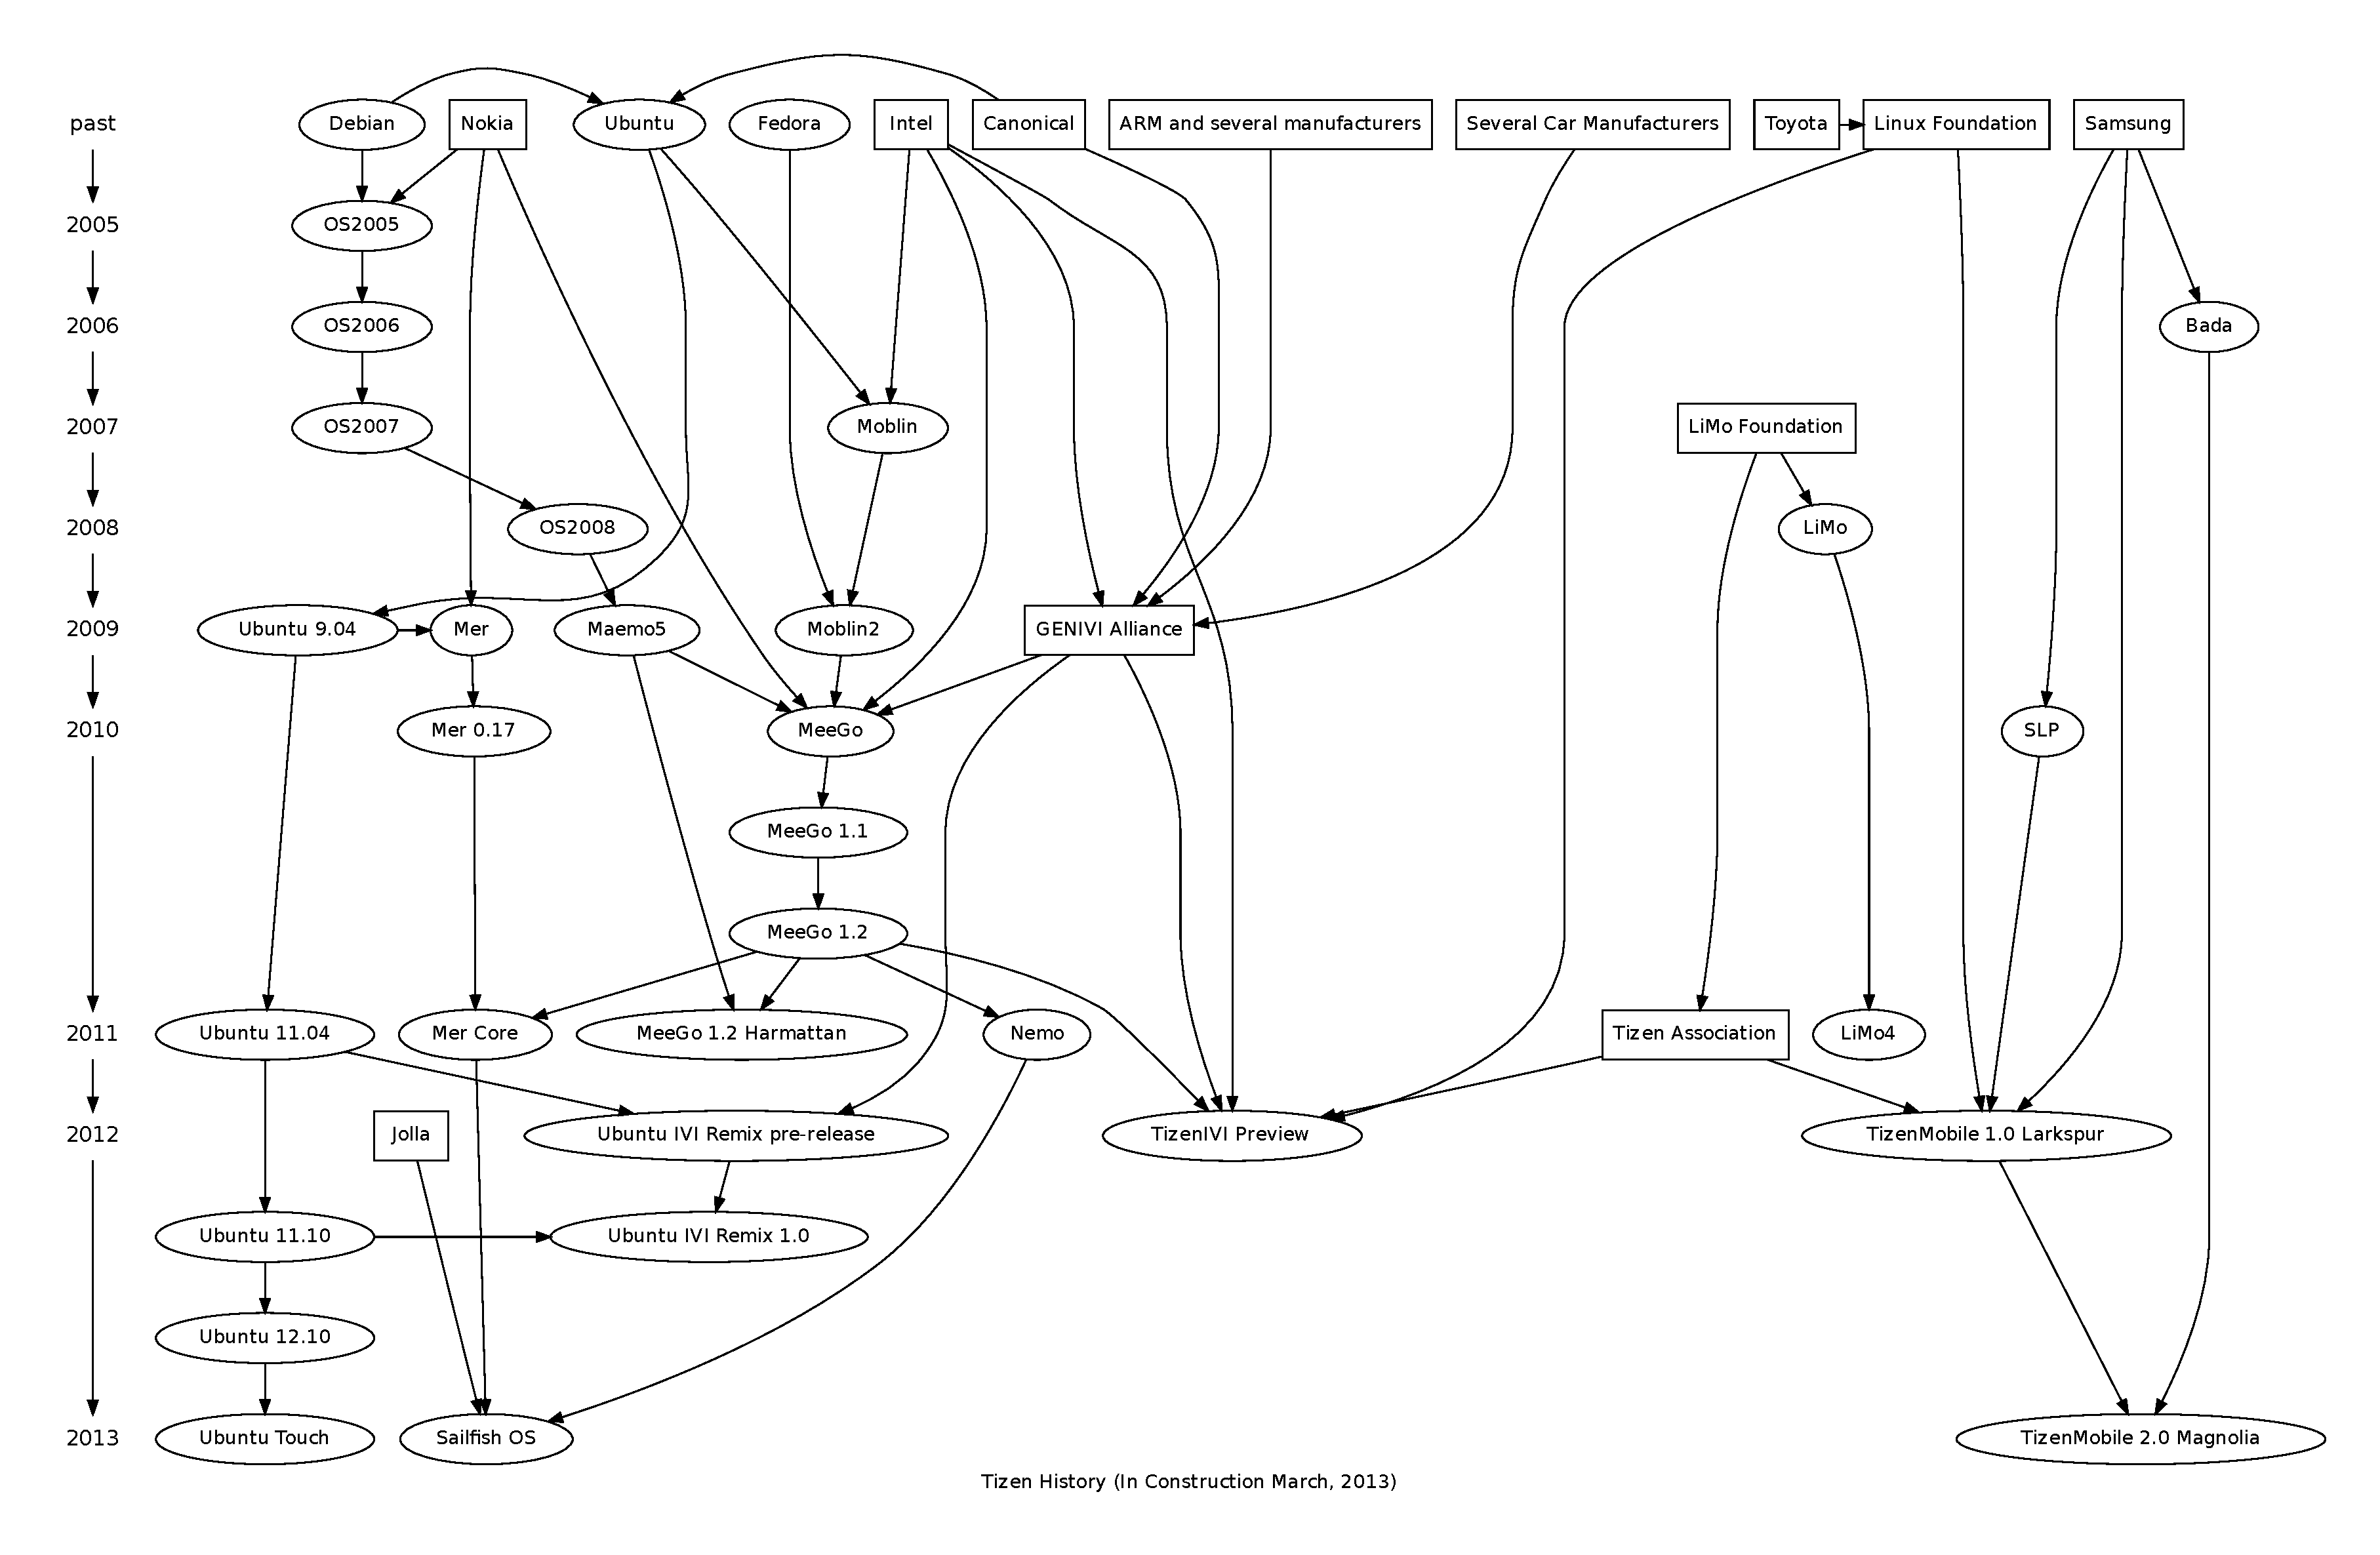
\includegraphics[height=.75\paperheight]{tizen-history}}
\end{tikzpicture}
%% \setlength{\unitlength}{1pt}
%% \begin{picture}(310,205)
%% \color{black}\thinlines
%% \uncover<2->{\put(262,182){\includegraphics[scale=.25]{ellip_p2985.eps}}} % Samsung
%% \uncover<3->{\put(262,182){\vector(-3, -4){20}}}
%% \uncover<3->{\put(215.5,142){\includegraphics[scale=.25]{ellip_p2985.eps}}} % LiMo Foundation
%% \uncover<4->{\put(251,102){\includegraphics[scale=.25]{ellip_p2985.eps}}} % SLP
%% \uncover<5->{\put(105,182){\includegraphics[scale=.25]{ellip_p2985.eps}}} % Intel
%% \uncover<6->{\put(93.5, 75.5){\includegraphics[scale=.25]{ellip_p2985.eps}}} % MeeGo
%% \uncover<7->{\put(120, 82){\vector(4, -1){85}}} % MeeGo
%% \uncover<8->{\put(206.5,62){\includegraphics[scale=.25]{ellip_p2985.eps}}} % Tizen Association
%% \uncover<9->{\put(245,49){\includegraphics[scale=.25]{ellip_p2985.eps}}} % Tizen 1.0
%% \uncover<10->{\put(264,9){\includegraphics[scale=.25]{ellip_p2985.eps}}} % Tizen 2.0
%% \put(0,0){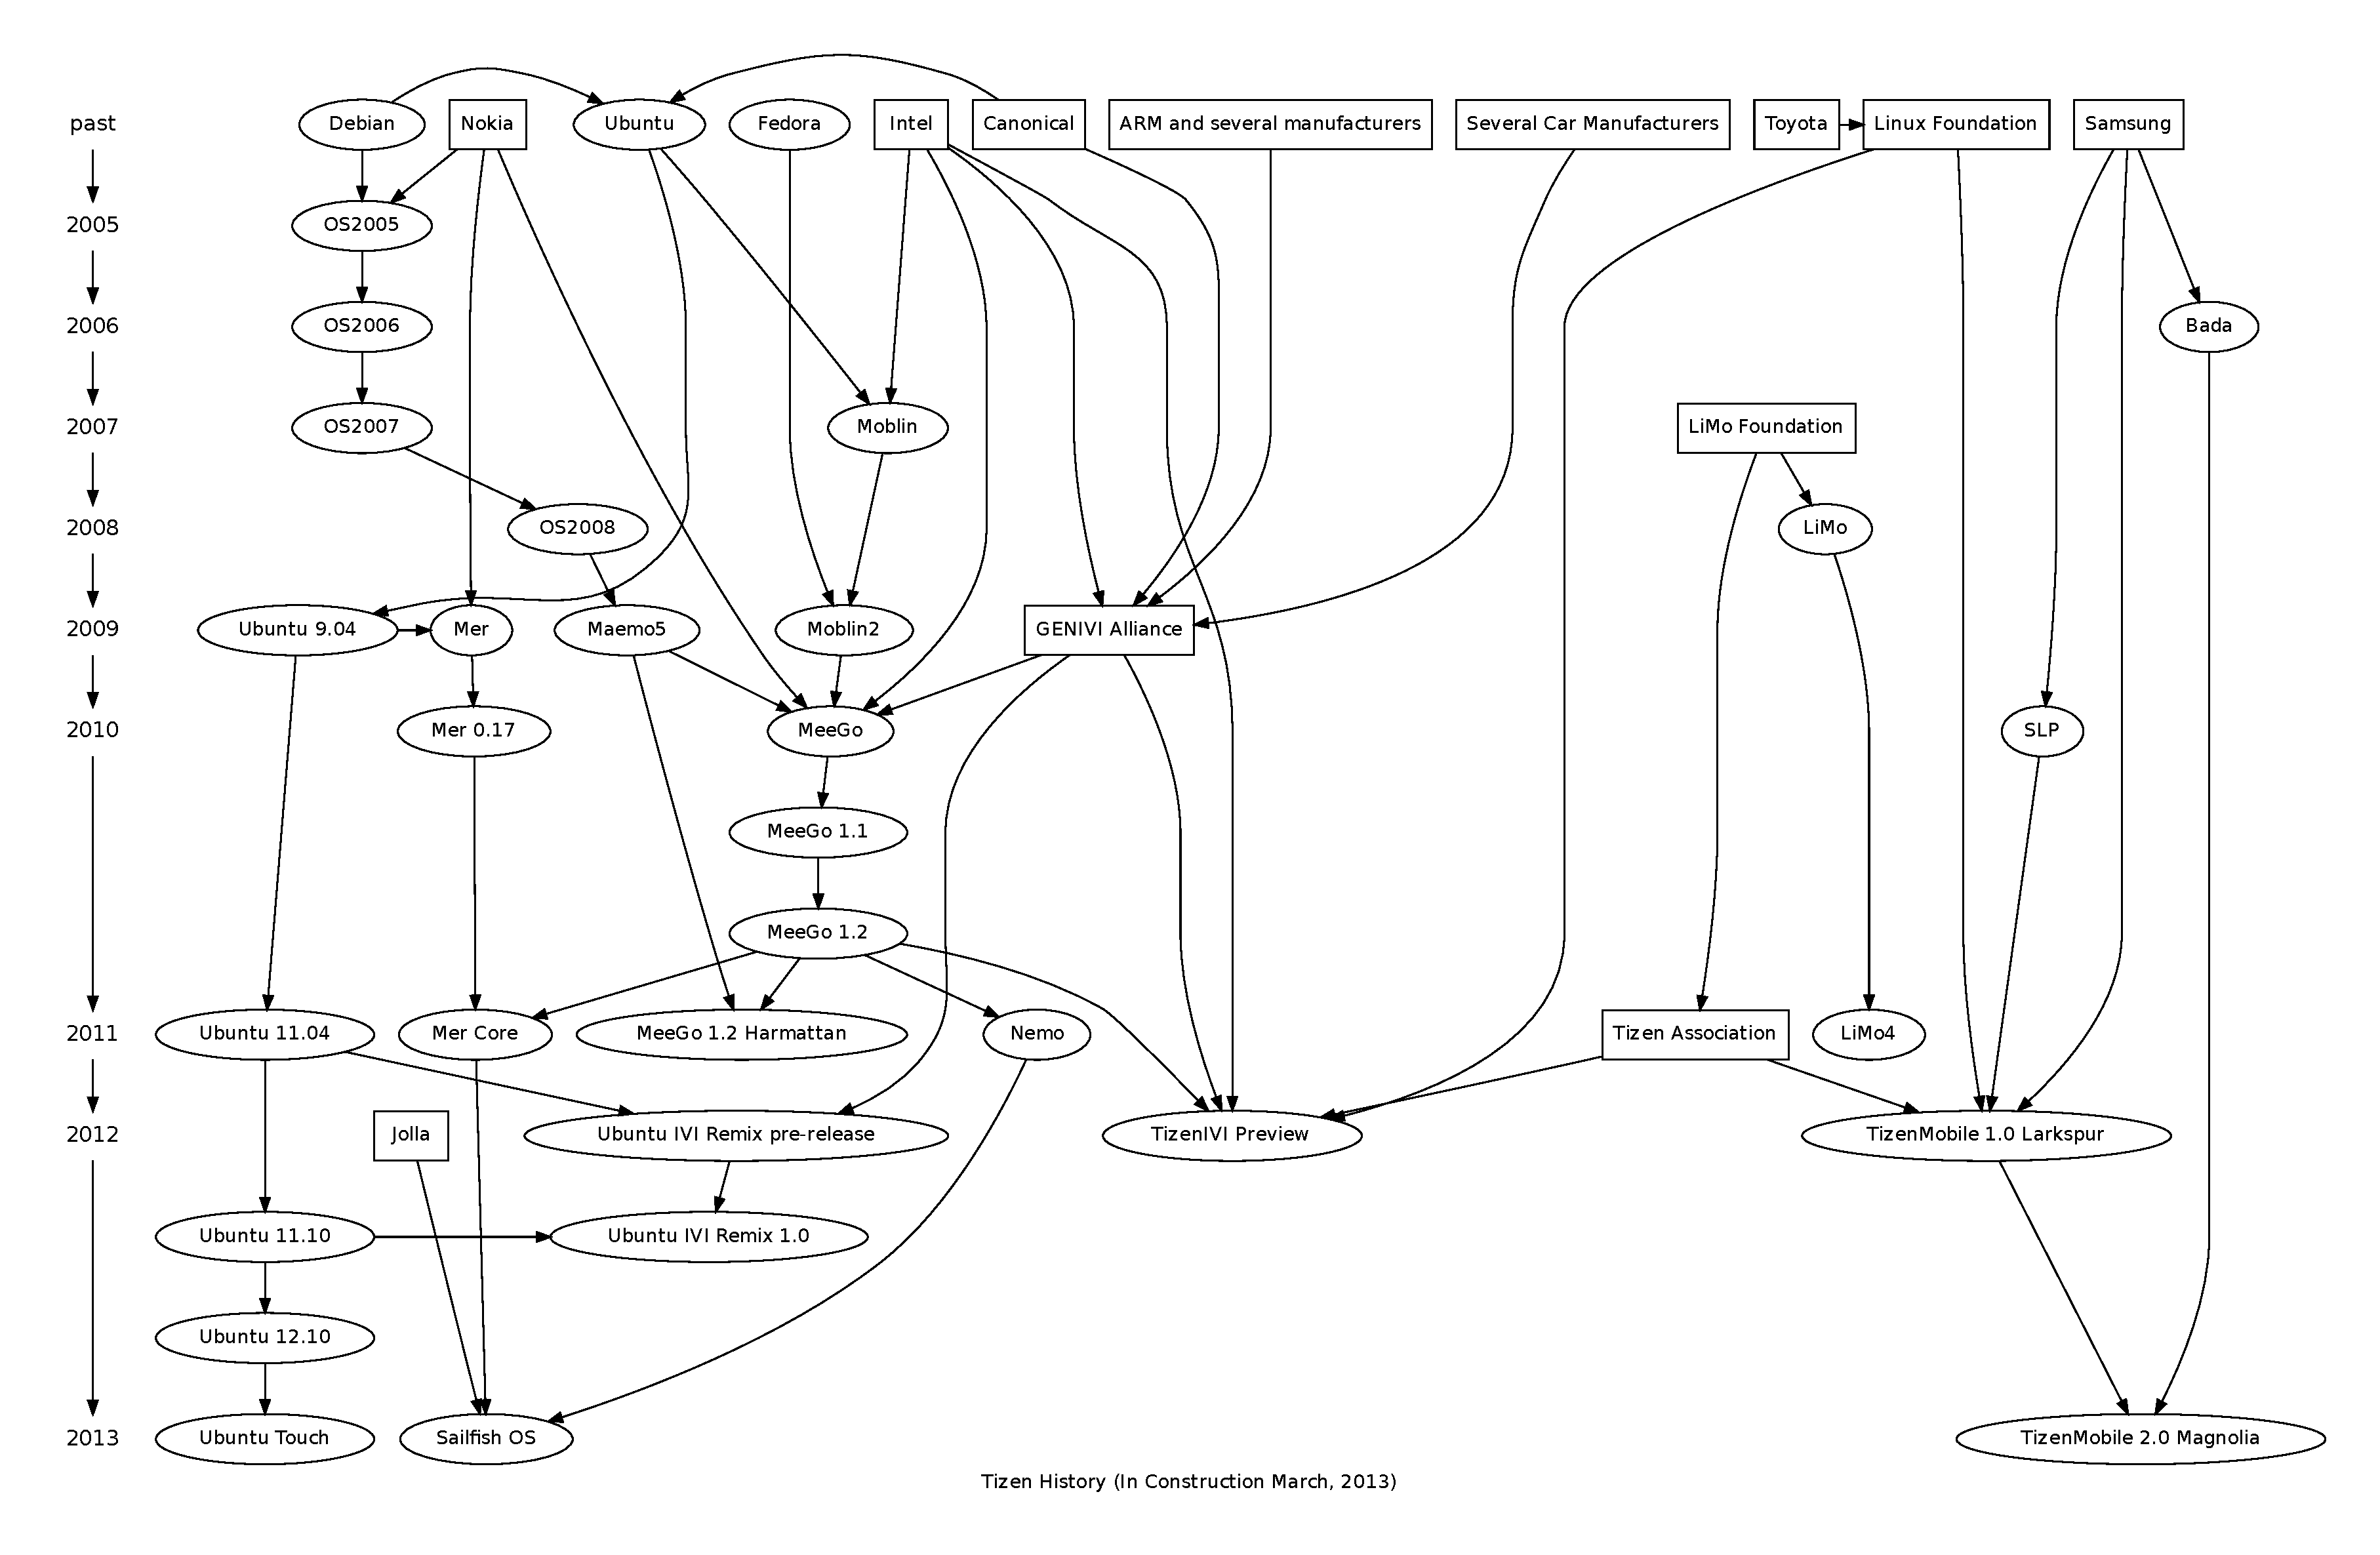
\includegraphics[width=1.2\paperheight,height=.8\paperheight]{tizen-history}}%
%% \end{picture}
\end{center}
\end{frame}
\begin{frame}[label=sec-2-4]{Tizen's origins, things to remember}
\begin{itemize}
\item LiMo $\to$ Tizen Association
\item Samsung + Intel
\item Tizen $\neq$ MeeGo
\item Tizen has got few bits from MeeGo
\begin{itemize}
\item Connman
\item oFono
\item BlueZ
\item RPM
\item staff
\end{itemize}
\item I assure you we are open. \url{http://www.tizen.org}
\end{itemize}

\note{T-33

The things I would like you to remember are:

\begin{itemize}
\item Tizen Association continues efforts of LiMo foundation
\item Samsung and Intel are the main contributors to Tizen
\item Tizen is not MeeGo although Intel brought some useful bits from it.
\end{itemize}


The first releases have been developed in a closed environment and
released afterwards. The development process of the 3.0 is fully
transparent. \url{http://www.tizen.org}}
\end{frame}

\section{Inside Tizen}
\label{sec-3}
\begin{frame}[label=sec-3-1]{Layers}
\begin{center}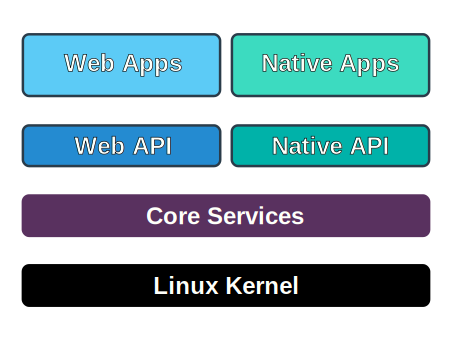
\includegraphics[height=.75\paperheight]{Architecture.eps}\end{center}
\note{T-32

Layers\ldots{} we like them don't we. The picture is pretty simple
while still being true, unbelivable.

\begin{itemize}
\item Kernel (\emph{mainline})
\item Core (GNU + Tizen)
\item APIs (Bada + WebRuntime)
\item Applications (C++ + HTML)
\end{itemize}

In my team we develop one of many parts of the Core layer. This is
what I know best and it isn't exposed directly to developers so I
would like to talk about it a little.}
\end{frame}
\begin{frame}[label=sec-3-2]{Tizen Core Services}
\begin{columns}
\begin{column}{0.5\textwidth}
\begin{itemize}
\item Application Framework
\item Base
\item Connectivity
\item Graphics \& UI
\item Location
\item Messageing
\end{itemize}

\end{column}

\begin{column}{0.5\textwidth}
\begin{itemize}
\item Multimedia
\item PIM
\item Security
\item System
\item Telephony
\item Web
\end{itemize}

\end{column}
\end{columns}

\note{Application Framework, Base, Connectivity, Graphics \& UI,
Location, Messageing, Multimedia, PIM, Security, System,
Telephony, Web}
\end{frame}
\begin{frame}[label=sec-3-3]{Base}
\begin{itemize}
\item A basic self-contained GNU/Linux userland
\item Boots to console with a login prompt
\item Toolchain
\item Support libraries
\begin{itemize}
\item database access
\item i18n
\item XML and others
\end{itemize}
\end{itemize}
\note{T-30

Although this part is completely invisible to the end-user and even
developers aren't supposed to be exposed to it to much it is
crucial that it works flawlessly. To make sure it does we put here
as much free software as possible.

\begin{itemize}
\item gnu/linux userland
\item systemd as init
\item gcc toolchain
\item libraries, pretty much the same you find on a desktop linux.
\end{itemize}}
\end{frame}

\begin{frame}[label=sec-3-4]{Application Framework}
\begin{itemize}
\item Application state management
\item Pre-defined services
\item Notifications
\item Package management
\item Alarm/time management
\end{itemize}

\note{\begin{itemize}
\item Pre-defined like dialer
\item Notifications about system events: batteries, orientation (sensors)
\end{itemize}}
\end{frame}
\begin{frame}[label=sec-3-5]{Network \& Connectivity}
\begin{itemize}
\item TCP/IP connection
\item Bluetooth
\item HTTP
\item NFC
\item Wi-Fi
\end{itemize}

\note{\begin{itemize}
\item connectivity ConnMan
\item Bluetooth (BlueZ)
\item HTTP: libsoup, curl
\item NFC
\item Wi-Fi: direct
\end{itemize}}
\end{frame}

\begin{frame}[label=sec-3-6]{Graphics \& UI}
\begin{itemize}
\item X11
\item OpenGL
\item Enlightenment Foundation Libraries (EFL)
\item Input methods
\end{itemize}

\note{\begin{itemize}
\item Tizen graphics stack is based on X11, we are experimenting with Wayland
\item OpenGL
\item EFL present, several applications use it but not an official API
\item Input Methods
\end{itemize}}
\end{frame}
\begin{frame}[label=sec-3-7]{Location}
\begin{itemize}
\item GeoClue
\begin{itemize}
\item GPS
\item WiFi
\item 3G
\item GeoIP
\item Geocoding
\end{itemize}
\end{itemize}

\note{Location services are based on GeoClue. Currently the following
we've got plugins to do the following tasks.

GPS, WiFi, 3G/Network, GeoIP, Geocoding}
\end{frame}
\begin{frame}[label=sec-3-8]{Messaging}
\begin{itemize}
\item SMS, MMS
\item Email
\item Push
\end{itemize}
\note{Samsung is going to provide application developers with a
cloud-part of the push. You need to register your application and
you can use Samsung's cloud to forward messages for it.}
\end{frame}
\begin{frame}[label=sec-3-9]{Multimedia}
\begin{itemize}
\item Video
\item Audio
\item Camera
\item Audio Policy
\item 3D Audio
\end{itemize}

\note{Multimedia framework is ready to support hardware codecs for
Video. There are ongoing works to support audio.

Audio policy, scenarios provided by PulseAudio.}
\end{frame}

\begin{frame}[label=sec-3-10]{PIM}
\begin{itemize}
\item Contacts
\item Calendar
\item Accounts
\item Synchronisation
\end{itemize}
\end{frame}
\begin{frame}[label=sec-3-11]{Security}
\begin{itemize}
\item Access control
\item Certificates
\item Secure storage
\item Cryptography
\item DRM
\end{itemize}

\note{\begin{itemize}
\item Tizen is the first commercial-grade system to use SMACK

Certificats, Secure storage, Cryptography, DRM
\end{itemize}}
\end{frame}
\begin{frame}[label=sec-3-12]{System}
\begin{itemize}
\item Sensors
\item Power management
\item System settings
\end{itemize}
\end{frame}
\begin{frame}[label=sec-3-13]{Telephony}
\begin{itemize}
\item Telephony services
\item Network communication
\item SIM management
\end{itemize}
\end{frame}
\begin{frame}[label=sec-3-14]{Web}
\begin{itemize}
\item WebKit: layout + rendering
\item WebRuntime
\end{itemize}

\note{\begin{itemize}
\item You can find my colleagues' contribution at WebKit.org
\item Saturday, 2013-09-14 09:00 — \emph{Webruntime in Tizen}, Janusz Majnert (T2)
\end{itemize}}
\end{frame}
\begin{frame}[label=sec-3-15]{API}
\begin{columns}
\begin{column}{0.5\textwidth}

\begin{itemize}
\item HTML5
\item Native C++ (Bada)
\end{itemize}

\end{column}

\begin{column}{0.5\textwidth}
\begin{itemize}
\item Tizen Common
\item Application
\item Communication
\item Content
\item Input/Output
\item Social
\item System
\item User Interface
\end{itemize}

\end{column}
\end{columns}
\note{T-20

Those services are available through proper APIs to both native
and HTML5 applications.

Thre are two official sets of APIs: HTML5 and C++. The former
based on WebRuntime the latter is a Linux port of Samsung's OSP
Bada framework. The former is cross platform the latter is not. If
you want to know more about HTML5 runtime we will meet at Janusz
Majnert's talk on Saturday.

You may ask what about: EFL, Qt? The former, although present, is
not a part of the official API. The latter isn't there, officially.
Qt has been ported to Tizen and Jarosław Staniek will tell you
more about it on Saturday too.}
\end{frame}
\section{Tizen and others}
\label{sec-4}
\note{No numbers.
I don't want to speak about numbers on the following slides. The
numbers are different everytime you look at them. Besiedes, most of
you porbably, know them better than I do. I'd like to show a
qualitive comparison between the most common mobile operatiing
systems\ldots{} and Tizen.

This is my own view and I am not an application developer. My
conclusions may not apply to you if you are one. If it happens so,
I will be glad to discuss it during Q\&A part.}
\begin{frame}[label=sec-4-2]{The players}
\begin{itemize}
\item Android
\item iOS
\item RIM (BlackBerry OS, QNX)
\item Windows Phone
\item Tizen
\end{itemize}
\note{T-18

\begin{itemize}
\item Android: Aparently Google wants too much leaving little for:
manufacturers, operators (developers?).
\item iOS: to me it seems like it too much depend on fashion/trend.
\item Windows Phone: that's becoming quite interesting
\item Tizen: new kid on the block. The first mobile devices are going
to be released by the end of this year.
\end{itemize}}
\end{frame}
\begin{frame}[label=sec-4-3]{Areas of applications}
\begin{itemize}
\item Android: pretty much anything
\item iOS: iStuff
\item RIM: Blackberry phones and tablets
\item Windows Phone: Nokia (mostly)
\item Tizen: pretty much anything
\end{itemize}

\note{T-16}
\end{frame}

\begin{frame}[label=sec-4-4]{Software development}
\begin{itemize}
\item Android: Java
\item iOS: ObjectiveC
\item RIM: Native (C/C++), HTML5, Adobe AIR, Android (BB10)
\item Windows Phone: .NET, C++
\item Tizen: Native (C++), HTML5, (Android via ACL)
\end{itemize}
\note{T-14

\begin{itemize}
\item iOS Developer license to run a code on a device
\item RIM: most versatile
\item ACL: Andoroid APK to Tizen TPK with a little help from OpenMobile
\end{itemize}}
\end{frame}

\begin{frame}[label=sec-4-5]{Platform development}
\begin{itemize}
\item Android: open (?)
\item iOS: closed
\item RIM: closed
\item Windows Phone: closed
\item Tizen: open (!)
\end{itemize}

\note{T-12

Android dev. model is technicaly open. There are community
driven distributions like CyanogenMod. However, Android does not
run on the mainline Linux kernel. Google, driven by NIH
syndrome, wrote a lot of code just to make sure they don't have
any GPL code in userland.

Tizen: Is becoming an opensource project. Tizen is going to run on
mainline kernel because we push our changes upstream. As I
mentioned before there we've got GPL userland and it's not a
problem for us. If some piece software needs modification to meet
our needs we work with its developers to push changes upstream and
get them back with the latest version.}
\end{frame}
\begin{frame}[label=sec-4-6]{Software distribution}
\begin{itemize}
\item Android: Play Store
\item iOS: App Store
\item RIM: BlackBerry World
\item Windows Phone: Windows Phone Store
\item Tizen: Tizen Store (?)
\end{itemize}

\note{T-10

\begin{itemize}
\item Android: Play or not, no problem.
\item iOS: I do not follow the news and I remember that in the
beginning application development was quite risky as one could
find one day that Apple didn't like an app that took three
months of full time development and was supposed to be the
beginning of a start-up.
\item Tizen store is open for developers. How it is going to work? TBD
\end{itemize}}
\end{frame}

\section{Q\&A}
\label{sec-5}
\begin{frame}[label=sec-5-1]{Thank you}
Łukasz Stelmach <l.stelmach@samsung.com>
\end{frame}

\begin{frame}[label=sec-5-2]{More About Tizen}
\begin{itemize}
\item Friday, 2013-09-13
\begin{itemize}
\item 15:15 — \emph{Creating a Tizen Application}, Kamil Grondys (T1)
\item 17:30 — \emph{HTML5} Features, Wojciech Bielawski (T2)
\end{itemize}
\item Saturday, 2013-09-14
\begin{itemize}
\item 09:00 — \emph{Webruntime in Tizen}, Janusz Majnert (T2)
\item 11:15 — \emph{Porting Qt to a new Smarthone for Fun and Fame},
Jarosław Staniek (T1)
\item 11:15 — Solution for Tizen/, Michał Knapiński
and Michal Pawluk (T2)
\end{itemize}
\end{itemize}
\end{frame}
% Emacs 24.2.1 (Org mode 8.1.1)
\end{document}
